\documentclass[12pt]{article}
\usepackage[export]{adjustbox}
\usepackage[utf8]{inputenc}
\usepackage{graphicx}
\usepackage{caption}
\usepackage{subfig}
\usepackage{lipsum}
\usepackage{geometry}
\geometry{
 a4paper,
 total={170mm,257mm},
 left=20mm,
 top=20mm,
 }
%\usepackage{biblatex}
%\addbibresource{references.bib}



\title{COP290: User Registration App}
\author{Aayan Kumar (2014CS10201) \\ Shreyan Gupta (2014CS10485) \\ Vaibhav Bhagee (2014CS50297) }

\begin{document}
\maketitle

The application takes in the details of a team vis-a-vis name of the team, name of the members and their entry numbers and registers the team online, on the given server.

\section{User Interface}

\begin{center}
\begin{tabular}{c c c}
     
\begin{minipage}[t]{.3\textwidth}
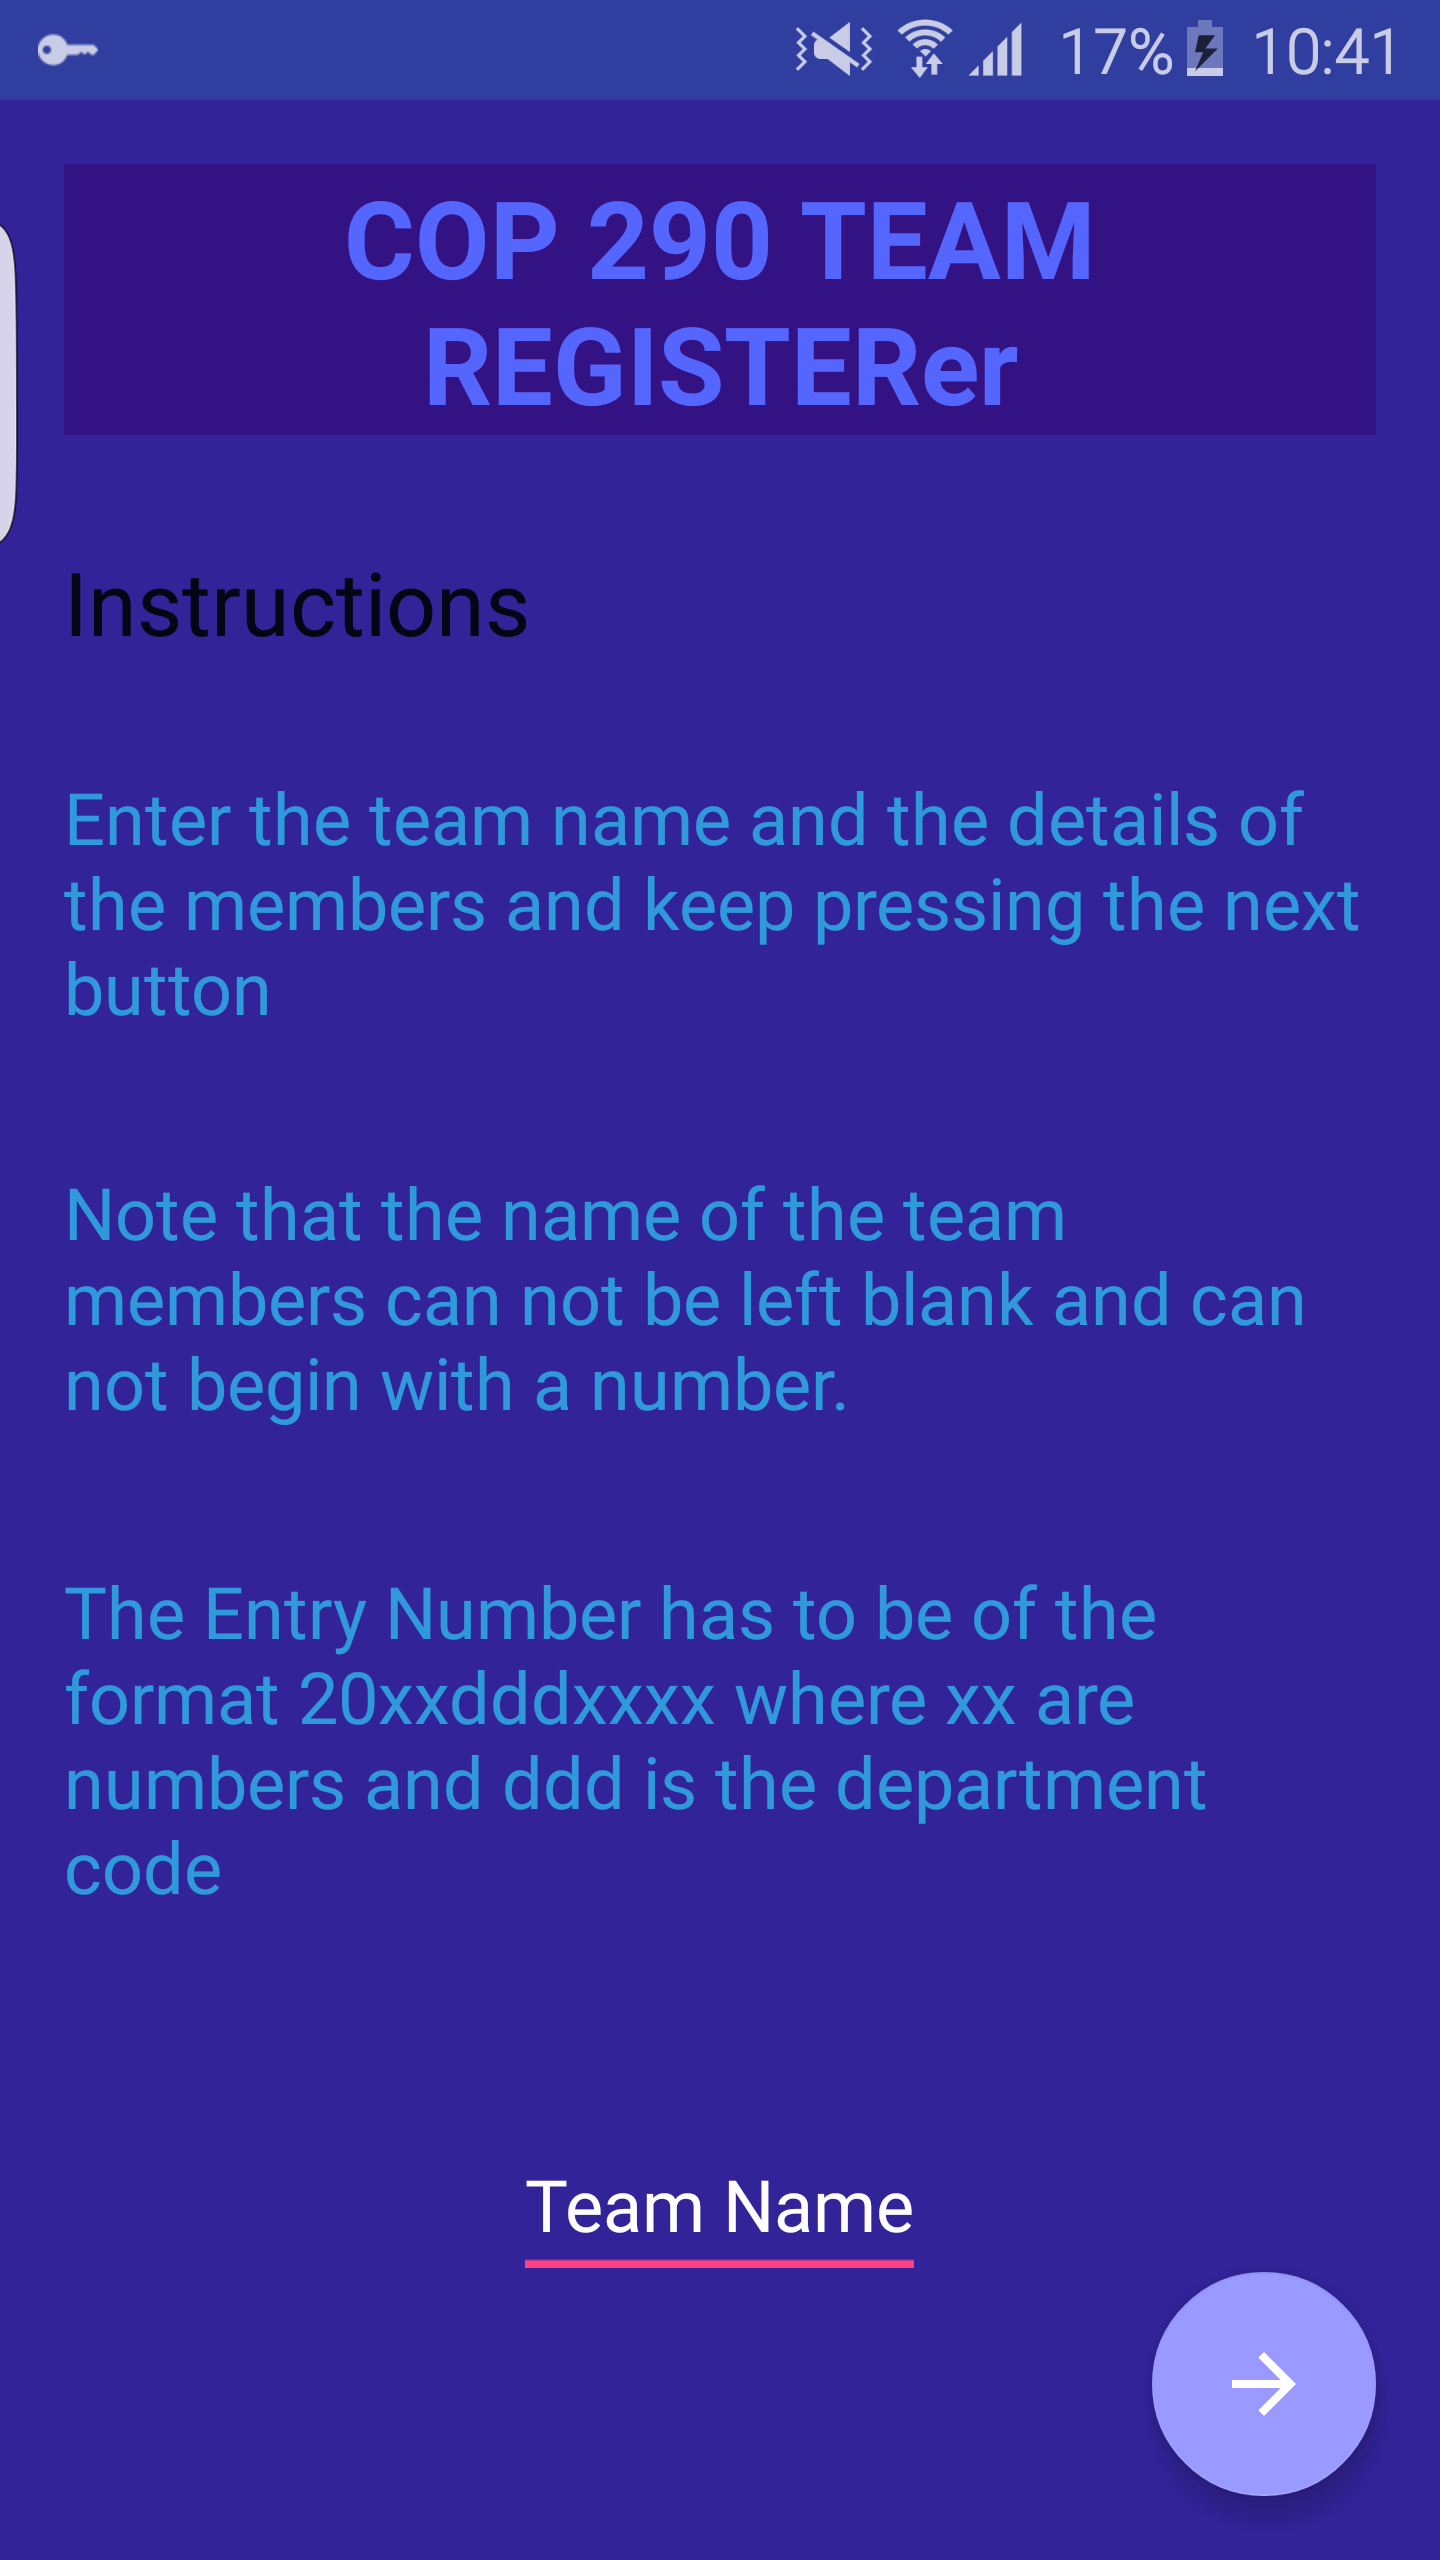
\includegraphics[width=\textwidth]{./Intro_Page}
\captionsetup{justification=raggedright, singlelinecheck=false}
\captionof{figure}{Introduction Page}
\end{minipage}%
% \begin{minipage}[t]{.1\textwidth}
&
% \end{minipage}
\begin{minipage}[t]{.3\textwidth}
 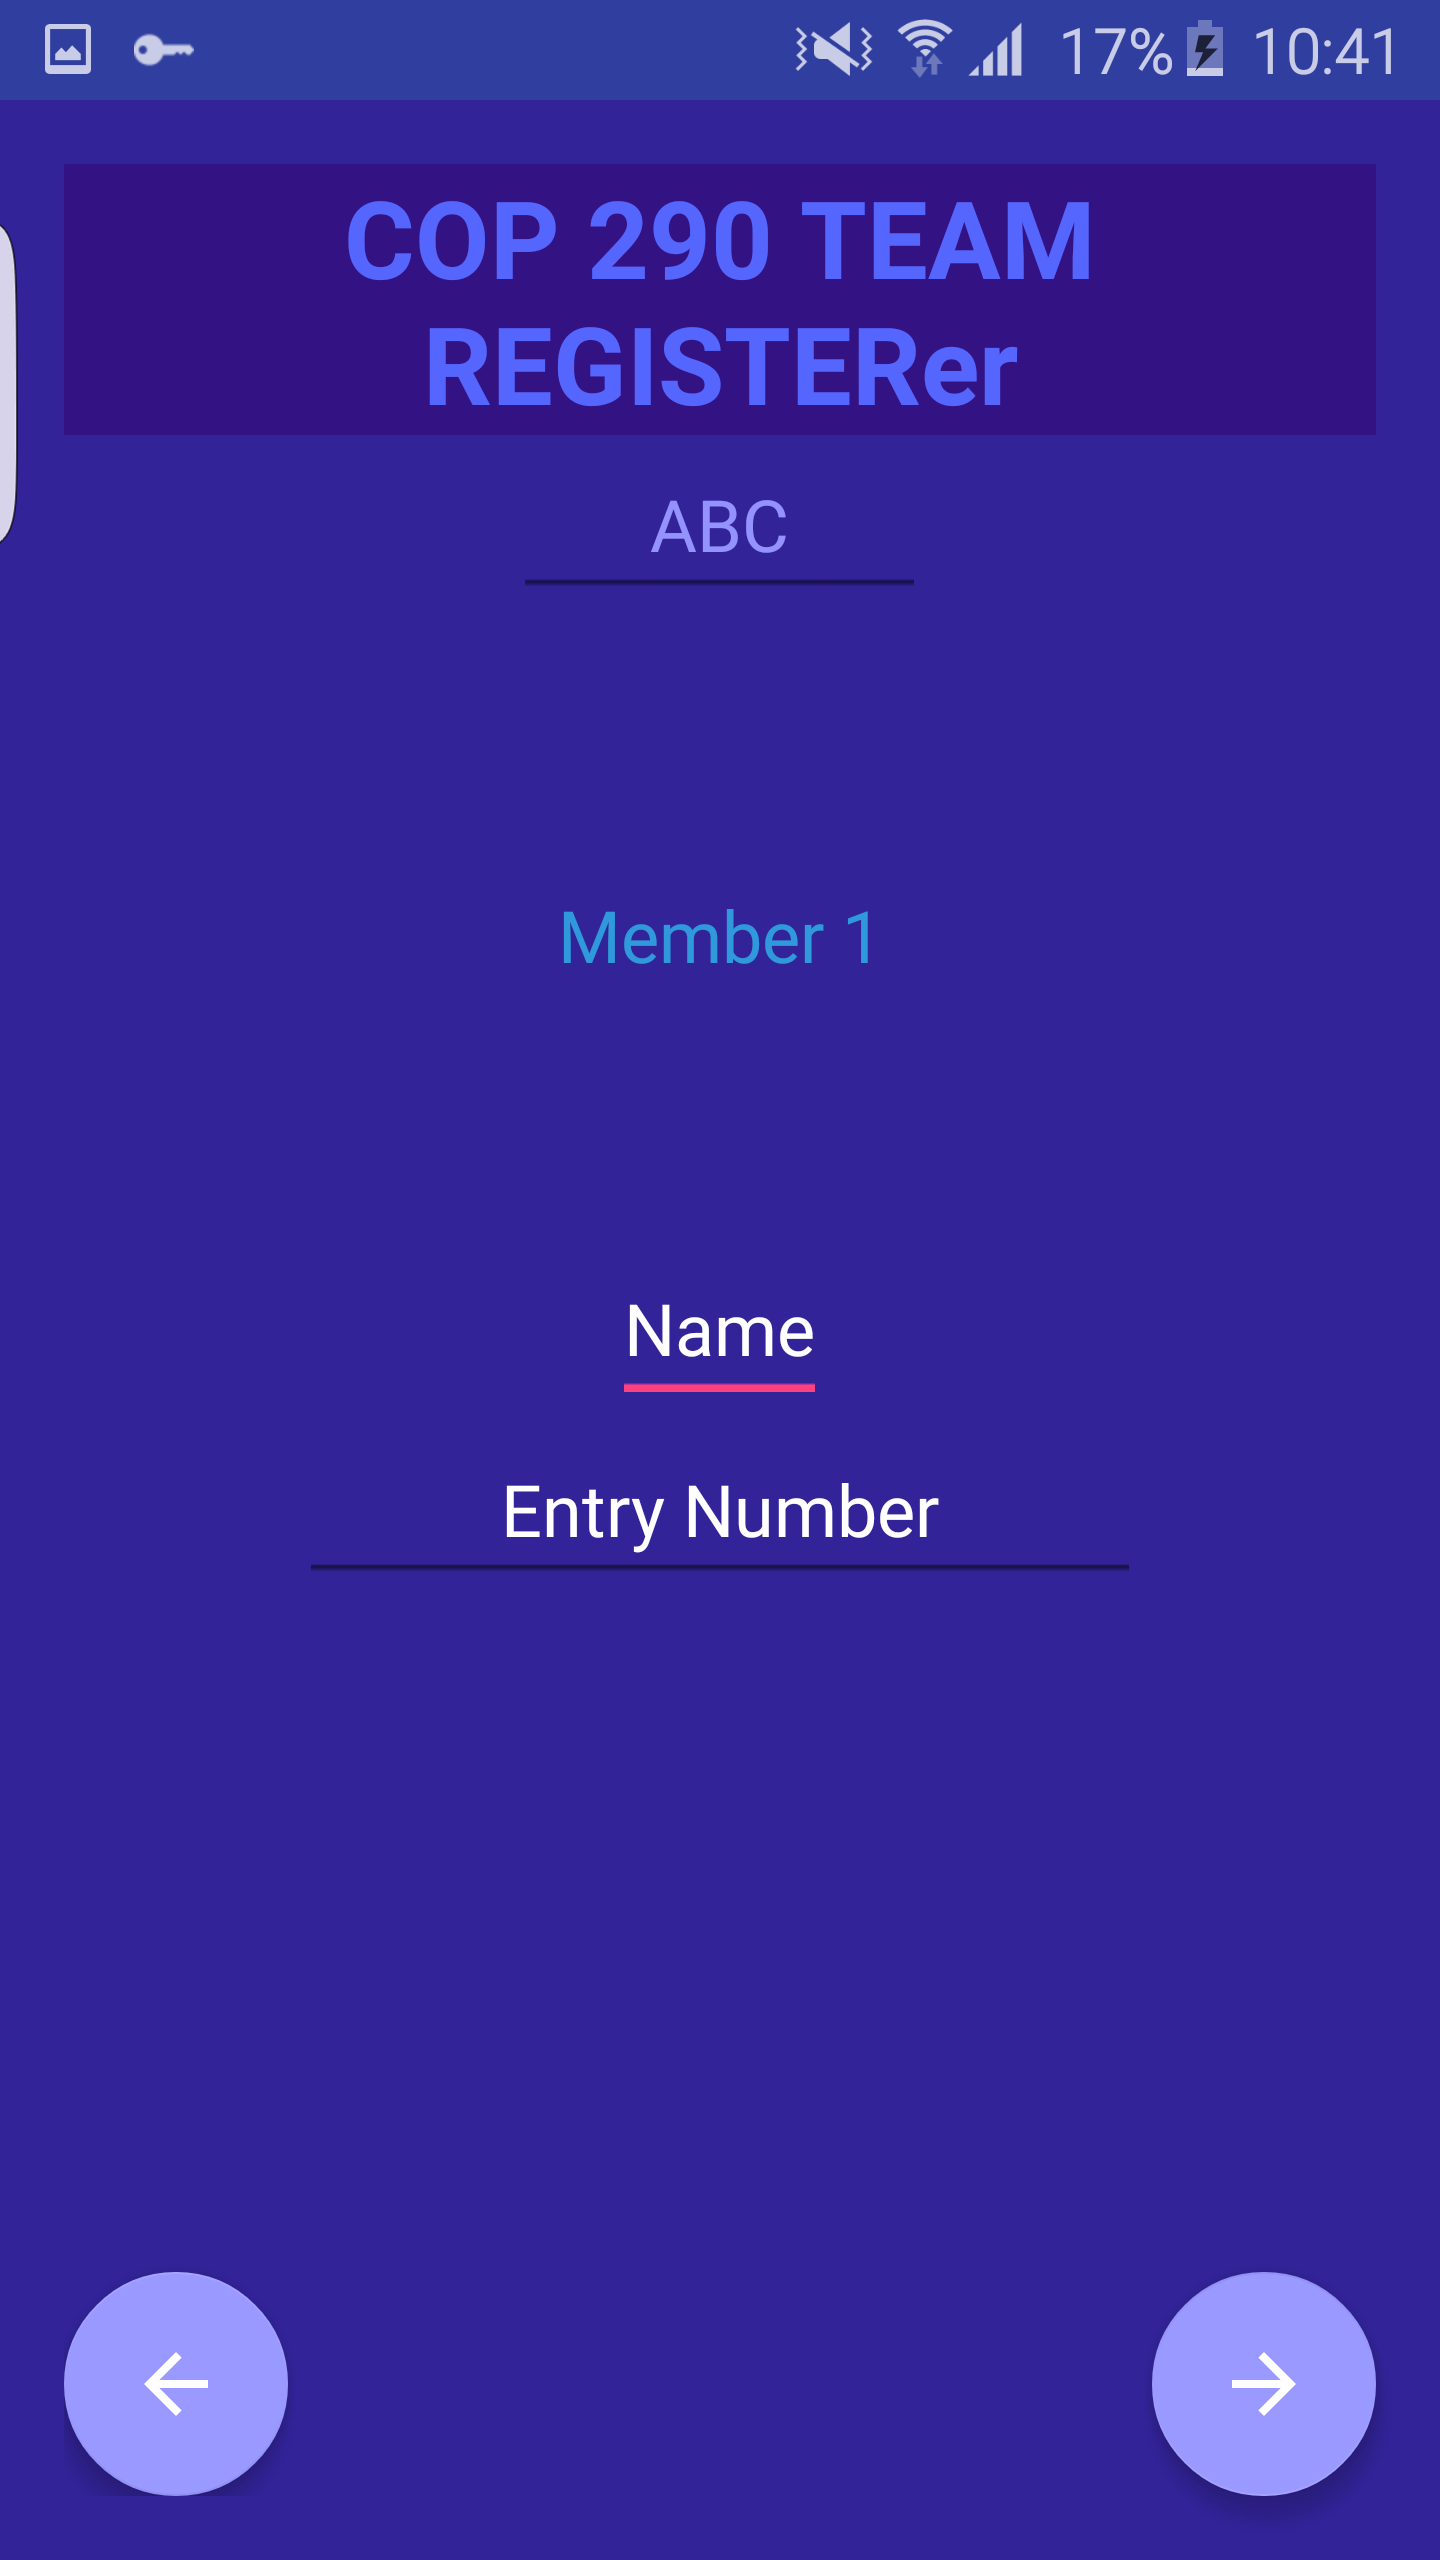
\includegraphics[width=\textwidth]{./User_Details}
 \captionsetup{justification=raggedright, singlelinecheck=false}
\captionof{figure}{Entering User Details}
\end{minipage}
% \begin{minipage}[t]{.1\textwidth}
& 
% \end{minipage}
\begin{minipage}[t]{.3\textwidth}
 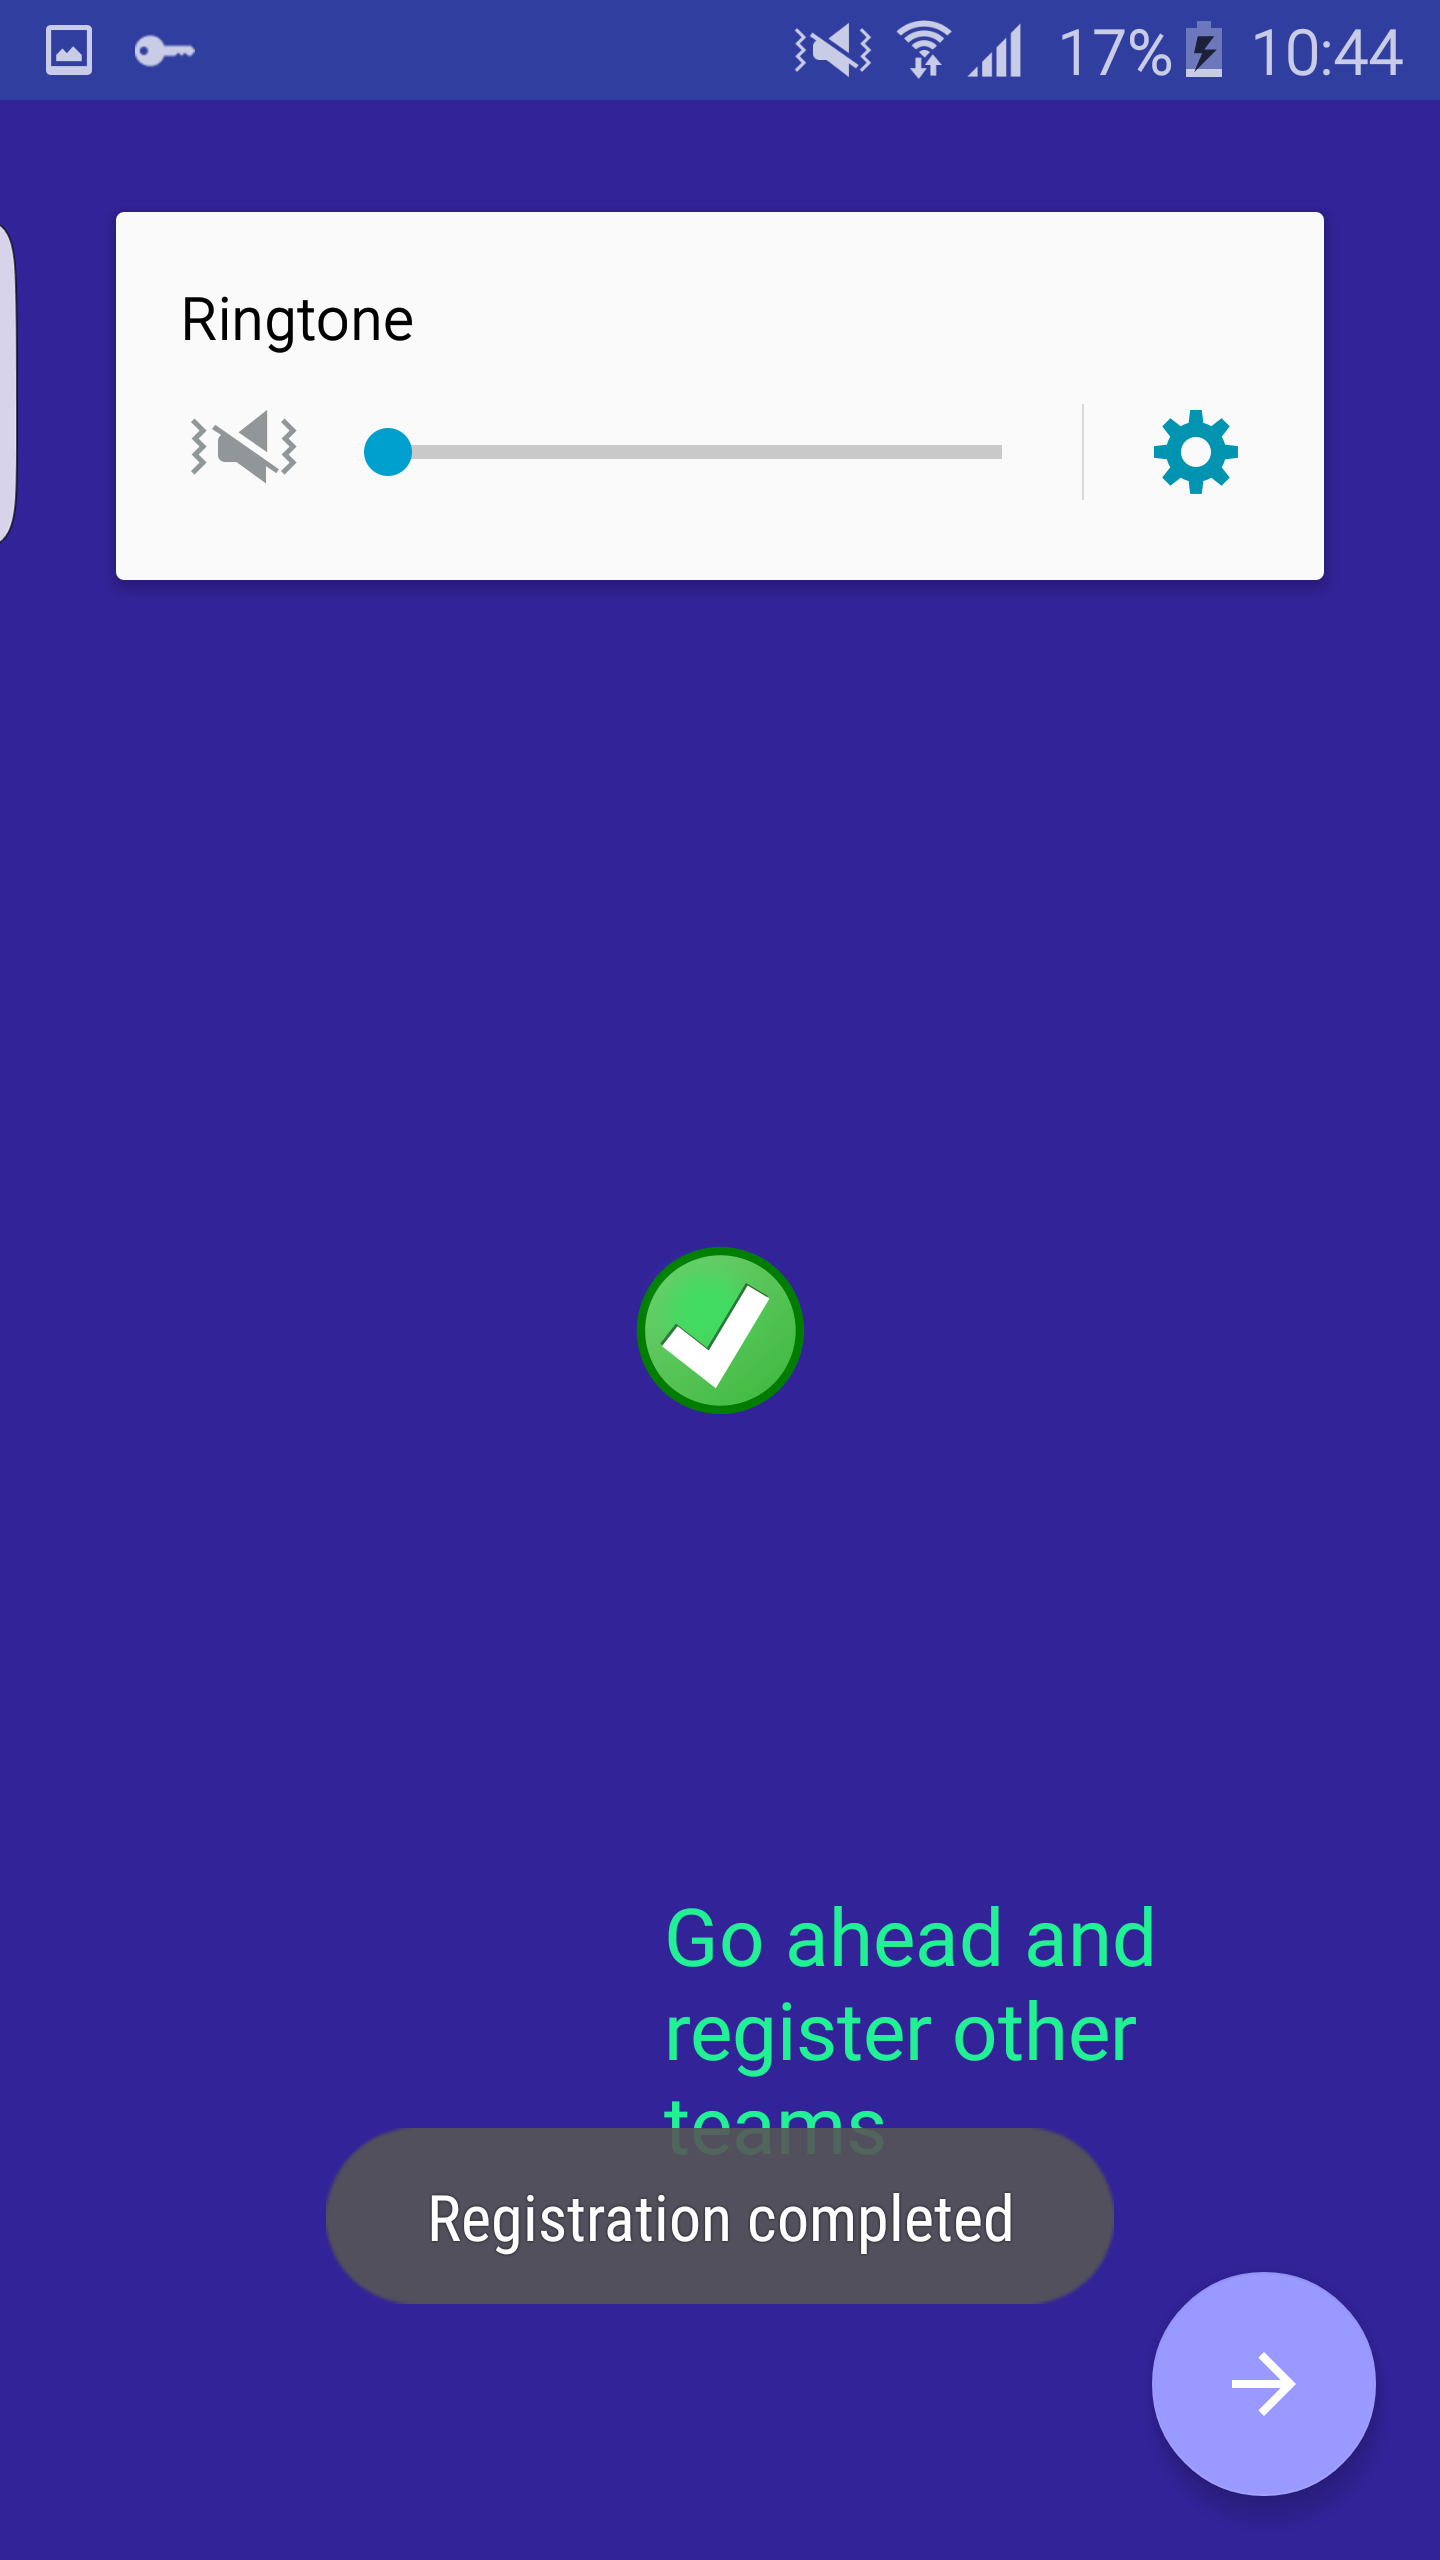
\includegraphics[width=\textwidth]{./On_Successful_Registration}
 \captionsetup{justification=raggedright, singlelinecheck=false}
\captionof{figure}{On Successful Registration}
\end{minipage}
  \\
\end{tabular}
\end{center}

\begin{itemize}
\item The following screens are encountered:
    \begin{itemize}
        \item A \textbf{Home Screen} which displays instructions to the user and asks for the team name
        \item 3 different \textbf{User-Details-Entering-Screen} in which each team member enters his/her name and entry number is the specified format
        \item A \textbf{Validation Screen} which shows whether the registration was successful or not
    \end{itemize}
    
\newpage
\item \begin{itemize}
    \item Animations have been added to improve overall user experience. Transitions are inserted as the App moves from one Page to another.
    \item The user can easily switch between screens using the forward and backward buttons on all the screens. 
    
    \end{itemize}
\item 
\begin{itemize}
    \item As the user enters the relevant details and presses the forward button, the appropriate data validations are imposed and and error message in form of an Alert is flashed if the data is found to be of an incorrect format. The user can move to the next page only if the data entered is properly validated. 
\item On the final page where the last User's details are implemented, the Send button send the registration details to the server for validation. A toast is used to display the response message of the server.
\end{itemize}
\end{itemize}

\section{Implementation Details~\cite{developer_android}~\cite{stack_overflow}}

\begin{itemize}
\item Each data entry like team name, member names are stored in separate Strings. On each page, when the navigation buttons are pressed, the user information is extracted from the text boxes and, along with the data collected from previous pages, put into a Bundle and passed onto the next activity.
\item Button clicks are detected using event handlers. These wait until the button click is detected, after which they immediately executed.
\item Multiple pages have been created using separate activities. Intents are used to navigate from one Activity to another. 
\item The three basic data validations which are used in this application are basically, checking for empty string, checking for proper format of names and of entry numbers. The validations have been enforced using JAVA RegEx (Regular Expressions).~\cite{regex_test}.
	\begin{itemize}
		\item The entries for the names should begin with a capital or a small letter followed by any number of letters/spaces/underscores
		\item The entries for the Entry Numbers of the team members should be of the form \textbf{20YNDDDNNNN} where Y is either 0 or 1, N is a number from 0 to 9 and DDD are the various undergraduate department codes of IIT Delhi. Thus the details of entry years from 2000 to 2019 along with the correct department codes followed by a four digit number will be considered as valid.
	\end{itemize}
\item The android library volley was used to interact with the server. The data was posted on the server through an HTTP-POST request~\cite{post_volley} with the data being sent as a Map from String to String. The string response obtained from the server was parsed and displayed as a Toast.  
~\cite{android_network_tutorial}.
\end{itemize}

The code for the project is being maintained in this repository~\cite{git_tutorial}: \\\centerline{{\em https://github.com/vaibhavbhagee/Assignment-0-src.git}}.

\newpage

\bibliographystyle{abbrv}
\medskip
\bibliography{references}
\end{document}